\documentclass{article}

\textwidth=6.5in
\textheight=8.5in
\voffset=-54pt
\oddsidemargin=0in
\evensidemargin=0in
\setlength{\parskip}{8pt}
\setlength{\parindent}{0pt}

\usepackage{workbook}

\usepackage[]{handout}

\begin{document}

\begin{center}
  \large\textsc{Problem Set 23 - Properties of the Definite Integral}
  
      \pspace{12pt}
  \begin{problemonly}\large Name: \rule{5cm}{0.15mm}\\ \end{problemonly}
\end{center}

For help with these problems, you may wish to read pp. 738-741 and 747-755 in Gottlieb.

\begin{enumerate}
\item 

\begin{grading}
10 points: 3/3/4.
\end{grading}

  Evaluate the following. (\emph{Hint: Think graphically.})  
  \probonly{}
    \begin{enumerate}
    \item
      \begin{problem}[\vfill]
        $\displaystyle \int_2^0 x\,dx$
      \end{problem}

      \begin{solution}
        $\displaystyle \int_2^0 x\,dx = -\int_0^2 x\,dx = \boxed{-2}$ by
        visualizing $\displaystyle \int_0^2 x\,dx$ as the following signed
        area:
        \begin{center}
          \begin{tikzpicture}
            \begin{axis}[cycle list=black, axis equal=true, xtick={0, 2},
              ytick={0, 2}, width=2.5in]
              \addplot+[domain=0:2, plusarea] {x} \closedcycle;
              \addplot+[domain=-0.5:2.5] {x} node[left] {$y = x$};
            \end{axis}
          \end{tikzpicture}
        \end{center}
      \end{solution}

    \item
      \begin{problem}[\vfill]
        $\displaystyle \int_4^{-1} \left( |x - 1| - 2 \right) dx$
      \end{problem}

      \begin{solution}
        First, we can rewrite this:
        \begin{align*}
          \int_4^{-1} \left( |x - 1| - 2 \right) dx &=
          -\int_{-1}^4 \left( |x - 1| - 2 \right) dx \\
          &= - \left( \int_{-1}^4 |x - 1|\,dx - \int_{-1}^4 2\,dx \right)
        \end{align*}
        We can visualize 
        $\displaystyle \int_{-1}^4 |x -1|\,dx$ and $\displaystyle
        \int_{-1}^4 2\,dx$ as the following signed areas: 
        \begin{center}
          \begin{tabular}{ccc}
            \begin{tikzpicture}
              \begin{axis}[cycle list=black, axis equal=true, xtick={-1, 1, 4},
                ytick=\empty, width=2.5in]
                \addplot+[domain=-1:4, plusarea] {abs(x-1)} \closedcycle;
                \addplot+[domain=-1.5:4.5] {abs(x-1)} node[left] {$y = |x-1|$};
              \end{axis}
            \end{tikzpicture} &
            \hspace{1in} &
            \begin{tikzpicture}
              \begin{axis}[cycle list=black, axis equal=true, xtick={-1, 4},
                ytick={2}, width=2.5in, ymin=0]
                \addplot+[domain=-1:4, plusarea] {2} \closedcycle;
                \addplot+[domain=-1.5:4.5] {2};
              \end{axis}
            \end{tikzpicture} \\
            $\displaystyle \int_{-1}^4 |x - 1|\,dx$ & & $\displaystyle
            \int_{-1}^4 2\,dx$
          \end{tabular}
        \end{center}
        Therefore, $\displaystyle \int_{-1}^4 |x - 1|\,dx = \frac{13}{2}$
        and $\displaystyle \int_{-1}^4 2\,dx = 10$, so $\displaystyle
        \int_4^{-1} \left( |x - 1| - 2 \right) dx = - \left( \frac{13}{2}
          - 10 \right) = \boxed{\frac{7}{2}}$.
      \end{solution}

    \item
      \begin{problem}[\vfill\newpage]
        $\displaystyle \int_{-1}^1 \left( 2\sqrt{1-x^2} + 7 \right) dx$
      \end{problem}

      \begin{solution}
        We can rewrite this as
        \begin{align*}
          \int_{-1}^1 \left( 2\sqrt{1-x^2} + 7 \right) dx &= \int_{-1}^1 2
          \sqrt{1 - x^2}\,dx + \int_{-1}^1 7\,dx \\
          &= 2 \int_{-1}^1 \sqrt{1 - x^2}\,dx + \int_{-1}^1 7\,dx \\
          \intertext{We can visualize the integrals $\displaystyle
            \int_{-1}^1 \sqrt{1 - x^2}\,dx$ and $\displaystyle \int_{-1}^1
            7\,dx$ as signed area (remember that $y = \sqrt{1 - x^2}$ is
            the equation of the top half of the circle with radius 1 whose
            center is the origin), to figure out that:}
          &= 2 \left( \frac{1}{2} \pi \right) + 14 \\
          &= \boxed{\pi + 14}
        \end{align*}
      \end{solution}
    \end{enumerate}
    \probonly{}

\item 
\begin{grading}
5 points. Deduct at least 2 points if they evaluate part (d) and claim that one of the other integrals is impossible.
\end{grading}

Suppose $\displaystyle \int_{0}^{5} f(t)\,dt =10$. Evaluate four out
    of the five expressions below (you do not have enough information to
    evaluate the remaining one).

    \probonly{ \raggedcolumns}
      \begin{enumerate}
      \item
        \begin{problem}[\vfill]
          $\displaystyle \int_{0}^{5}7f(t)\,dt$
        \end{problem}

        \begin{solution} % Jason Bland
          This equals $\displaystyle 7 \int_0^5 f(t) \, dt = \boxed{70}$.
        \end{solution}

      \item
        \begin{problem}[\vfill]
          $\displaystyle \int_{0}^{5}\left(f(t)+7 \right)\,dt$
        \end{problem}

        \begin{solution} % Jason Bland
          We can split up the integral as $\displaystyle \int_0^5 f(t)
          \, dt + \int_0^5 7 \, dt = 10 + 7 \cdot 5 = \boxed{45}$.

          (We can visualize $\displaystyle \int_0^5 6\,dt$ as a signed
          area to evaluate it.) 
        \end{solution}

      \item
        \begin{problem}[\vfill]
          $\displaystyle \int_{0}^{5}f(t)\,dt + 7$
        \end{problem}

        \begin{solution} % Jason Bland
          This is just $10 + 7 = \boxed{17}$.
        \end{solution}

      \item
        \begin{problem}[\vfill]
          $\displaystyle \int_{0}^{5}7f(t+7)\,dt$
        \end{problem}

        \begin{solution}
          There is not enough information.  The graph of $f(t + 7)$ is
          the graph of $f(t)$ shifted left by $7$ units, so the behavior
          of $f(t + 7)$ on $[0, 5]$ has nothing to do with the behavior
          of $f(t)$ on $[0, 5]$.
        \end{solution}

      \item
        \begin{problem}[\vfill\newpage]
          $\displaystyle \int_{-7}^{-2}7f(t+7)\,dt$
        \end{problem}

        \begin{solution} 
          The graph of $f(t + 7)$ is the graph of $f(t)$ shifted left by
          $7$ units, so the signed area under $f(t)$ from $t = 0$ to $t
          = 5$ is the same as the signed area under $f(t + 7)$ from $t =
          -7$ to $t = -2$.  That is, $\displaystyle \int_{-7}^{-2} f(t +
          7)\,dt = \int_0^5 f(t)\,dt$.  Therefore, $\displaystyle
          \int_{-7}^{-2} 7 f(t + 7) \, dt = 7 \int_{-7}^{-2} f(t +
          7)\,dt = 7 \int_0^5 f(t) \, dt = \boxed{70}$.
        \end{solution}

      \end{enumerate}
      \probonly{}

\item 
%Inspired by Gottlieb 22.4.5

\begin{grading}
5 points: 1/1/3
\end{grading}

  \begin{enumerate}
  \item
    \begin{problem}[\vfill]
      Suppose $a < b$.  Fill in the blank below with either $\geq$ or
      $\leq$; explain your reasoning clearly.
      \[ \int_{a}^{b} |f(t) |\,dt \quad \fitb{0.35in}{} \quad
      \left|\int_{a}^{b} f(t)\,dt\right| \]
      \emph{Hint:} Try drawing pictures of some different functions $f$.
    \end{problem}

    \begin{solution} 
      Here's an example of the difference between $\displaystyle \int_a^b
      f(t)\,dt$ and $\displaystyle \int_a^b |f(t)|\,dt$:
      \begin{center}
        \begin{tabular}{ccc}
          \begin{tikzpicture}[declare
            function={f(\x)=\x*(\x-1)*(\x-3)*(\x-4)*(\x-5.1);}] 
            \begin{axis}[hide y axis, xtick={0.5, 4.5}, xticklabels={$a$,
                $b$}, cycle list=black, ymin=-15, ymax=15, width=2.5in] 
              \addplot+[domain=0.5:1, plusarea] {f(x)} \closedcycle;
              \addplot+[domain=1:3, minusarea] {f(x)} \closedcycle;
              \addplot+[domain=3:4, plusarea] {f(x)} \closedcycle;
              \addplot+[domain=4:4.5, minusarea] {f(x)} \closedcycle;
              \addplot+[domain=0.25:4.75] {f(x)};
              \draw (axis cs: 0.25, 15) node[anchor=north west] {$y =
                f(t)$}; 
            \end{axis}
          \end{tikzpicture}
          &&
          \begin{tikzpicture}[declare
            function={f(\x)=abs(\x*(\x-1)*(\x-3)*(\x-4)*(\x-5.1));}] 
            \begin{axis}[hide y axis, xtick={0.5, 4.5}, xticklabels={$a$,
                $b$}, cycle list=black, ymin=-15, ymax=15, width=2.5in]
              \addplot+[domain=0.5:4.5, plusarea] {f(x)} \closedcycle;
              \addplot+[domain=0.25:4.75, samples=91] {f(x)};
              \draw (axis cs: 0.25, 15) node[anchor=north west] {$y =
                |f(t)|$}; 
            \end{axis} 
          \end{tikzpicture} \\
          $\displaystyle \int_a^b f(t)\,dt$ & \hspace{1in} &
          $\displaystyle \int_a^b |f(t)|\,dt$           
        \end{tabular}
      \end{center}
      As we can see, both integrals involve the same-sized regions, but in
      $\displaystyle \int_a^b |f(t)|\,dt$, every region contributes
      positive signed area.  In $\displaystyle \int_a^b f(t)\,dt$, some
      regions may contribute positive signed area while others contribute
      negative signed area; therefore, even when we take the absolute
      value of $\displaystyle \int_a^b f(t)\,dt$, it can never be bigger
      than $\displaystyle \int_a^b |f(t)|\,dt$.  That is, $\boxed{
        \int_a^b |f(t)| \, dt \geq \left| \int_a^b f(t) \, dt \right|}$.
    \end{solution}

  \item
    \begin{problem}[\vfill]
      Under what circumstances will the two expressions be equal?
    \end{problem}

    \begin{solution} % Jason Bland
      This will happen if the graph of $y = f(t)$ lies either entirely
      above the $x$-axis or entirely below it; that is, if $f(t) \geq 0$
      on $[a, b]$ or $f(t) \leq 0$ on $[a, b]$.  (In other words, $f$
      doesn't change sign on $[a, b]$.)
    \end{solution}

  \item Suppose that $f(t)$ gives the velocity of a raccoon who is
    wandering back and forth along a bicycle path.  Consider the three
    expressions
    \begin{equation*}
      \int_{a}^{b} f(t)\,dt, 
      \quad 
      \int_{a}^{b} |f(t) |\,dt,
      \quad \text{ and }\quad
      \left|\int_{a}^{b} f(t)\,dt\right|.
    \end{equation*}

    \begin{enumerate}
    \item
      \begin{problem}[\stretch{0.5}]
        Which expression gives the net change in the raccoon's position
        from time $a$ to time $b$?
      \end{problem}

      \begin{solution} 
        The rate of change of position is velocity $f(t)$, so the net
        change in position is given by $\displaystyle \int_a^b f(t) \,
        dt$.
      \end{solution}

    \item
      \begin{problem}[\stretch{0.5}]
        Which expression gives the total distance the raccoon travels from
        time $a$ to time $b$?
      \end{problem}

      \begin{solution} 
        The rate of change of distance is \emph{speed}, which is $|f(t)|$.
        Therefore, $\boxed{ \int_a^b |f(t)| \, dt} = {}$ (distance
        traveled by time $b$) - (distance traveled by time $a$), which is
        exactly the distance the raccoon travels between time $a$ and time
        $b$.
      \end{solution}

    \item
      \begin{problem}[\nstretch{0.5}]
        The raccoon's average speed between time $a$ and time $b$ is the
        total distance it traveled divided by the time elapsed.  Write a
        mathematical expression giving the raccoon's average speed between
        time $a$ and time $b$.
      \end{problem}

      \begin{solution}
        We've already seen that the distance the raccoon travels between
        times $a$ and $b$ is $\displaystyle \int_a^b |f(t)|\,dt$, so
        \[ \text{(average speed between times $a$ and $b$)} =
        \frac{\text{distance traveled}}{\text{time elapsed}} =
        \boxed{\frac{\displaystyle \int_{a}^{b} |f(t) |\,dt }{b-a}}.\] 
      \end{solution}

    \end{enumerate}
  \end{enumerate}

\item 

\begin{grading}
20 points: 8/2/2/3/3/2.
\end{grading}

Let $f(t)=2t$. We'll look at two area functions, $A(x)$ and $B(x)$, where
  $$
  A(x) = \int^x_0 f(t)\,dt\qquad \text{and} \qquad B(x) = \int^x_3
  f(t)\,dt.
  $$
  \begin{enumerate}

  \item
Evaluate the following quantities.

    \begin{enumerate}
      \item
        \begin{problem}[\vfill]
          $A(2)$
        \end{problem}

        \begin{solution}
          $A(2)$ is just another way of writing $\displaystyle
          \int_0^2 f(t)\,dt$; by visualizing this as signed area, we see
          that it's equal to $\boxed{4}$. 
        \end{solution}

      \item
        \begin{problem}[\vfill]
          $A(-2)$
        \end{problem}

        \begin{solution}
          $A(-2)$ is just another way of writing $\displaystyle
          \int_{0}^{-2} f(t)\,dt$, which is the same as $-\displaystyle
          \int_{-2}^0 f(t)\,dt$.  By visualizing $\displaystyle
          \int_{-2}^0 f(t)\,dt$ as signed area, we see that it's equal to
          $-4$, so $A(-2) = - (-4) = \boxed{4}$. 
        \end{solution}

      \item
        \begin{problem}[\vfill]
          $B(1)$
        \end{problem}

        \begin{solution}
          $B(1)$ is just another way of writing $\displaystyle
          \int_{3}^1 f(t)\,dt$, which is the same as $- \displaystyle
          \int_1^3 f(t)\,dt = \boxed{-8}$ (again, we can visualize as
          signed area). 
        \end{solution}

      \item
        \begin{problem}[\vfill]
          $B(-2)$
        \end{problem}

        \begin{solution}
          $B(-2)$ is just another way of writing $\displaystyle
          \int_3^{-2} f(t)\,dt$, which is the same as $-\displaystyle
          \int_{-2}^3 f(t)\,dt = \boxed{-5}$. 
        \end{solution}

    \end{enumerate}

  \item
\begin{problem}[\nstretch{2}]
      Find a formula (not involving an integral) for $A (x)$, where $x
      \ge 0$. 
    \end{problem}

    \begin{solution}
      $A(x)$ is just another way of writing $\displaystyle \int_0^x
      f(t)\,dt$.  Since we're working with $x \geq 0$, we can visualize
      this integral as the following signed area:
      \begin{center}
        \begin{tikzpicture}[declare function={f(\x)=2*\x;}]
          \begin{axis}[cycle list=black, width=2in, height=2.5in, axis
            equal=true, xtick={3}, xticklabels={$x$}, ytick=\empty]            
            \addplot+[domain=0:3, plusarea] {f(x)} \closedcycle;
            \addplot+[domain=-1:4] {f(x)} node[left]{$y = 2t$};
          \end{axis}
        \end{tikzpicture}
      \end{center}
      This is the area of a triangle of width $x$ and height $2x$, so it's
      equal to $\frac{1}{2} (x) (2x) = \boxed{x^2}$. 
    \end{solution}

  \item
\begin{problem}[\stretch{2}]
      Does the formula you wrote in {{{{\#4}}(b)}} work
      for negative $x$?  Explain. 
    \end{problem}

    \begin{solution}
      \fbox{Yes.}  One example that we've already seen from
      {{{{\#4}}(a)}} is that $A(-2) = 4$, but we can
      look at this more generally.  If $x < 0$, then $A(x) =
      \displaystyle \int_0^x f(t)\,dt = - \int_x^0 f(t)\,dt$, and we can
      visualize $\displaystyle \int_x^0 f(t)\,dt$ as the following signed
      area:
      \begin{center}
        \begin{tikzpicture}[declare function={f(\x)=2*\x;}]
          \begin{axis}[cycle list=black, width=2in, height=2.5in, axis
            equal=true, xtick={-3}, xticklabels={$x$}, ytick=\empty]            
            \addplot+[domain=-3:0, minusarea] {f(x)} \closedcycle;
            \addplot+[domain=-4:1] {f(x)} node[pos=0, right]{$y = 2t$};
          \end{axis}
        \end{tikzpicture}
      \end{center}
      This triangle has width $-x$\footnote{For example, if $x = -2$, the
        triangle has width $2$, which is the same as $-x = - (-2)$.} and
      height $-2x$, so its area is $\frac{1}{2} (-x)(-2x) = x^2$.
      Therefore, the \emph{signed} area is $\displaystyle \int_x^0
      f(t)\,dt = - x^2$, and $\displaystyle \int_0^x f(t)\,dt = x^2$.       
    \end{solution}

  \item
    \begin{problem}[\stretch{2}]
      Find a formula (not involving an integral) for $B(x)$, where $x
      \ge 3$. Does your formula work for $x < 3$ as well?
    \end{problem}

    \begin{solution}
      $B(x) = \displaystyle \int_3^x f(t)\,dt$; if $x \geq 3$, we can
      visualize this integral as the following signed area:
      \begin{center}
        \begin{tikzpicture}[declare function={f(\x)=2*\x;}]
          \begin{axis}[cycle list=black, width=2in, height=2.5in, axis
            equal=true, xtick={5}, xticklabels={$x$}, ytick=\empty]            
            \addplot+[domain=3:5, plusarea] {f(x)} \closedcycle;
            \addplot+[domain=-1:6] {f(x)} node[left]{$y = 2t$};
          \end{axis}
        \end{tikzpicture}
      \end{center}
      An easy way to calculate the area of this trapezoid is to take the
      area under the graph from $0$ to $x$ and then subtract the area
      under the graph from $0$ to $3$.  That is, 
      \[ \int_3^x f(t)\,dt = \int_0^x f(t)\,dt - \int_0^3 f(t)\,dt =
      \boxed{x^2 - 9}.\] This works for all $x$, regardless of whether $x$
      is greater or less than $3$, because we found in
      {{{{\#4}}(b)}} and
      {{{{\#4}}(c)}} that $\displaystyle
      \int_0^x f(t)\,dt = x^2$ for all $x$.
    \end{solution}

  \item
    \begin{problem}[\stretch{2}]
      Graph the functions $A(x)$ and $B(x)$.  Describe the
      relationship between them.
    \end{problem}

    \begin{solution}
      This is just asking us to graph $A(x) = x^2$ (shown in red) and
      $B(x) = x^2 - 9$ (shown in blue):
      \begin{center}
        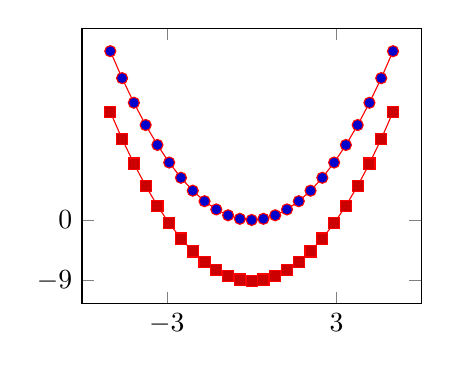
\begin{tikzpicture}
          \begin{axis}[ytick={0, -9}, xtick={-3, 3}, height=2in]
            \addplot+[domain=-5:5, red] {x^2};
            \addplot+[domain=-5:5] {x^2 - 9};
          \end{axis}
        \end{tikzpicture}
      \end{center}
      These two functions are vertical shifts of each other (if you shift
      $A(x)$ down 9 units, you get $B(x)$).
    \end{solution}

  \item
    \begin{problem}[\nstretch{2}]
      Differentiate $A (x)$ and $B(x)$.  How do these derivatives
      relate to $f$?
    \end{problem}

    \begin{solution}
      The derivatives are both equal to $f(x)=2x$.
    \end{solution}

  \end{enumerate}

\item 

\begin{grading}
8 points.
\end{grading}

  Here is the graph of a function $f$.  (The graph is composed of two
  straight line segments and one semicircle of radius 3.)  

  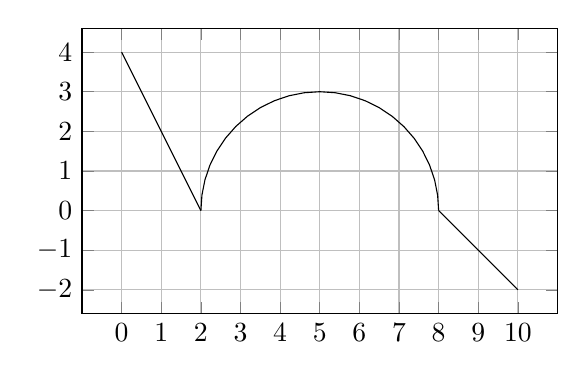
\begin{tikzpicture}
    \begin{axis}[xtick={0, 1, ..., 10}, ytick={-2, -1, ..., 4},
      grid=major, cycle list=black, axis equal=true, ymin=-2, ymax=4,
      clip=false, width=3in, height=2.05in, axis line style={shorten >=-8pt}]
      \addplot+[sharp plot] coordinates { (0, 4) (2, 0) };
      \addplot+[domain=0:180] ({3*cos(x) + 5}, {3*sin(x)}); 
      \addplot+[sharp plot] coordinates { (8, 0) (10, -2) };
    \end{axis}
  \end{tikzpicture}

  Let $A(x) = \displaystyle \int_0^x f(t)dt$ and let
  $B(x) = \displaystyle \int_5^x f(t)dt$. 
  Evaluate each of the following.

  \begin{center}
    \renewcommand{\arraystretch}{3}
    \begin{tabular}{>{$\displaystyle}l<{$} | >{$\displaystyle}l<{$}}
      \hline
      A(2) = \probonly{\text{\hspace{1in}}} 
      \solonly{\boxed{\int_0^2 f(x)\,dx = 4}}  &
      B(2) = \probonly{\text{\hspace{1in}}} 
      \solonly{\boxed{\int_5^2 f(x)\,dx = -\frac{9}{4}\pi}}
      \\ \hline
      A(5) = \solonly{\boxed{\int_0^5 f(x)\,dx = 4+\frac{9}{4}\pi}}  &
      B(5) = \solonly{\boxed{\int_5^5 f(x)\,dx = 0}}  \\ 
      \hline
      A(8) = \solonly{\boxed{\int_0^8 f(x)\,dx = 4+\frac{9}{2}\pi}}  &
      B(8) = \solonly{\boxed{\int_5^8 f(x)\,dx = \frac{9}{4}\pi}}  \\ 
      \hline
      A(10) = \solonly{\boxed{\int_0^{10} f(x)\,dx = 2+\frac{9}{2}\pi}}
      &
      B(10) = \solonly{\boxed{\int_5^{10} f(x)\,dx 
      = \frac{9}{4}\pi-2}}
      \\
      \hline
    \end{tabular}    
    \renewcommand{\arraystretch}{1}
  \end{center}

  \begin{problem}[\vfill\newpage]
    Do you see any relationship between $A(x)$ and $B(x)$?  Can
    you explain this relationship?
  \end{problem}

  \begin{solution}
    Looking at the examples so far, you may notice that $A(x)$ is
    always $4+\frac{9}{4}\pi$ more than $B(x)$; that is, 
    it appears that $A(x)
    = 4 + \frac{9}{4}\pi B(x)$.  
    We can use properties of the definite integral to see why this is true: 
    \begin{align*}
      \int_0^x f(t)\,dt &= \int_0^5 f(t)\,dt + \int_5^x f(t)\,dt \text{ by
        the Splitting Interval Property} \\
      \shortintertext{We can rewrite this:}
      A(x) &= \int_0^5 f(t)\,dt + B(x) \\
      \intertext{From the graph of $f$, we can see that $\displaystyle
        \int_0^5 f(t)\,dt = 4 + \frac{9}{4}\pi$, so}
      A(x) &= 4 + \frac{9}{4}\pi + B(x). 
    \end{align*}
  \end{solution}

% \item ({Problem Set 22}, {{\#5}})

% \emph{This problem is to help you get started with your exam review.}

%   ($\star$) On a dark night, a 6-foot-tall farmer is standing in his field
%   when he sees a UFO descending toward earth at a rate of 2 feet per
%   second.  Terrified, the farmer stands frozen in place while the UFO
%   shines a beam of light at the top of his head.  The farmer is 30 feet
%   away from the spot on the ground directly under the UFO.  When the UFO
%   is 24 feet over the field, the farmer's shadow is 10 feet long.

%   \begin{tikzpicture}
%     \pgfmathsetmacro{\angle}{30}    

%     \draw[green] (0, 0) -- (\angle: 5); 
%     %\draw (0, 0) -- (\angle:5) -- (\angle:5 |- 0, 0) -- (0, 0); %
%     \draw (-1, 0) -- ({5*cos(\angle) + 1}, 0);
%     \draw ({1/tan(\angle)}, 0) node[above, inner sep=0pt]
%     {\includegraphics[height=1cm]{images/man}}; %
%     \draw (\angle:5) node{\includegraphics[width=30pt]{images/ufo}}; %
%   \end{tikzpicture}

%   \begin{enumerate}
%   \item
%     \begin{problem}
%       At this moment, how quickly is the length of the farmer's shadow
%       changing?  Be sure to say whether the shadow is getting longer or
%       shorter.
%     \end{problem}

%     \probonly{\emph{You may want to look back at
%           {{{Problem Set 4}, {{{{\#6}}(b)}}}} and the follow-up on
%           {{{the worksheet ``Related Rates''}}}.}}

%     \begin{solution}
%       \ideas{This is a related rates problem, so let's start by drawing
%         two pictures, a generic picture that applies at any time, and a
%         ``snapshot'' showing the situation at the time we care about.
%         We'll also label some variables in the generic picture.}

%       \begin{center}
%         \begin{tabular}{ccc}
%           \begin{tikzpicture}
%             \pgfmathsetmacro{\angle}{30}    

%             \draw[green] (0, 0) -- (\angle: 5); \draw (\angle:5) --
%             node[right] {24} (\angle:5 |- 0, 0) -- (0, 0); %
%             \draw ({1/tan(\angle)}, 0) node[above, inner sep=0pt]
%             {\includegraphics[height=1cm]{images/man}}; %
%             \draw (\angle:5)
%             node{\includegraphics[width=30pt]{images/ufo}}; %
%             \draw[decorate, decoration={brace, mirror}, yshift=-2pt] (0,
%             0) -- node[below, yshift=-2pt] {10} ({1/tan(\angle)}, 0); %
%             \draw[decorate, decoration={brace, mirror}, yshift=-2pt]
%             ({1/tan(\angle)}, 0) -- node[below, yshift=-2pt] {30}
%             ({5*cos(\angle)}, 0); %
%             \draw[decorate, decoration={brace, mirror}, xshift=6pt]
%             ({1/tan(\angle)}, 0) -- node[right, xshift=2pt] {6}
%             ({1/tan(\angle)}, 1);
%           \end{tikzpicture} &&
%           \begin{tikzpicture}
%             \pgfmathsetmacro{\angle}{30}    

%             \draw[green] (0, 0) -- (\angle: 5); \draw (\angle:5) --
%             node[right] {$h$} (\angle:5 |- 0, 0) -- (0, 0); %
%             \draw (\angle:5)
%             node{\includegraphics[width=30pt]{images/ufo}}; %
%             \draw[decorate, decoration={brace, mirror}, yshift=-2pt] (0,
%             0) -- node[below, yshift=-2pt] {$s$} ({1/tan(\angle)}, 0); %
%             \draw[decorate, decoration={brace, mirror}, yshift=-2pt]
%             ({1/tan(\angle)}, 0) -- node[below, yshift=-2pt] {30}
%             ({5*cos(\angle)}, 0); %
%             \draw ({1/tan(\angle)}, 0) -- node[right] {6}
%             ({1/tan(\angle)}, 1); %
%           \end{tikzpicture} \\
%           \emph{Snapshot} & \hspace{0.25in} & \emph{Generic} \\
%         \end{tabular}
%       \end{center}
%       Notice that we've labeled the UFO's height as $h$ and the length of
%       the farmer's shadow as $s$. 

%       \ideas{Next, we figure out what we know and what we want to know.}

%       \highlight{
%         \textbf{What we know:} $\frac{dh}{dt} = -2$ (negative because $h$
%         is decreasing)

%         \textbf{What we want to know:} $\frac{ds}{dt}$
%       }

%       \ideas{Now, we try to relate variables.  In this case, since the
%         rate we know is $\frac{d\bm{h}}{dt}$ and the rate we want to know
%         is $\frac{d\bm{s}}{dt}$, we try to relate $h$ and $s$.}

%       Using similar triangles, we get

%       \highlight{\textbf{Equation relating our variables:} $\displaystyle
%         \frac{6}{s} = \frac{h}{30 + s}$} 

%       \ideas{Once we have our relating equation, we can differentiate it.
%         Since we are looking for $\frac{ds}{d\bm{t}}$, we should
%         differentiate with respect to $t$.}

%       Let's first rewrite our equation so that we don't need the Quotient
%       Rule when differentiating (this step is not necessary, but it can
%       make the differentiation easier!).  Cross multiplying,
%       \begin{align*}
%         6 (30 + s) &= sh \\
%         180 + 6s &= sh \\
%         \shortintertext{Now, we'll differentiate:}
%         \frac{d}{dt} \left( 180 + 6s \right) &= \frac{d}{dt} (sh) \\
%         6 \frac{ds}{dt} &= \frac{ds}{dt} h + s \frac{dh}{dt} \\
%         \intertext{At the moment we care about, $h = 24$, $s = 10$, and
%           $\frac{dh}{dt} = -2$:}
%         6 \frac{ds}{dt} &= 24 \frac{ds}{dt} + 10 (-2) \\
%         -18 \frac{ds}{dt} &= -20 \\
%         \frac{ds}{dt} &= \frac{10}{9}
%       \end{align*}
%       So, the shadow is \fbox{getting longer at a rate of $\frac{10}{9}$
%         feet per second}.

%       \begin{checkanswer}
%         It should make sense intuitively that, as the UFO descends, the
%         man's shadow gets longer.
%       \end{checkanswer}
%     \end{solution}

%   \item
%     \begin{problem}
%       At the same moment, how quickly is the angle between the ground and
%       the UFO's beam of light changing?  (Be sure to say whether it's
%       increasing or decreasing, and include units in your answer.)
%     \end{problem}

%     \begin{solution}
%       Our snapshot picture is the same as before, but let's label the
%       angle we're interested in in our generic picture:
%       \begin{center}
%         \begin{tikzpicture}
%           \pgfmathsetmacro{\angle}{30}    

%           \draw[green] (0, 0) -- (\angle: 5); \draw (\angle:5) --
%           node[right] {$h$} (\angle:5 |- 0, 0) -- (0, 0); %
%           \draw (\angle:5)
%           node{\includegraphics[width=30pt]{images/ufo}}; %
%           \draw[decorate, decoration={brace, mirror}, yshift=-2pt] (0, 0)
%           -- node[below, yshift=-2pt] {$s$} ({1/tan(\angle)}, 0); %
%           \draw[decorate, decoration={brace, mirror}, yshift=-2pt]
%           ({1/tan(\angle)}, 0) -- node[below, yshift=-2pt] {30}
%           ({5*cos(\angle)}, 0); %
%           \draw ({1/tan(\angle)}, 0) -- node[right] {6} ({1/tan(\angle)},
%           1); %
%           \draw (12pt, 0) arc[radius=12pt, start angle=0, end
%           angle=\angle]; % 
%           \draw ({\angle/2}:16pt) node{$\theta$};
%         \end{tikzpicture}        
%       \end{center}

%       \highlight{
%         \textbf{What we know:} $\frac{dh}{dt} = -2$ and $\frac{ds}{dt} =
%         \frac{10}{9}$ 

%         \textbf{What we want to know:} $\frac{d\theta}{dt}$
%       }

%       In this case, we can relate $\theta$ to $s$, $h$, or both, since we
%       know both $\frac{dh}{dt}$ and $\frac{ds}{dt}$.  It looks simplest to
%       relate $\theta$ to $s$ using the small right triangle:

%       \highlight{\textbf{Equation relating our variables:} $\displaystyle
%         \tan \theta = \frac{6}{s}$}

%       Therefore,
%       \begin{align*}
%         \frac{d}{dt} (\tan \theta) &= \frac{d}{dt} \left( \frac{6}{s}
%         \right) \\
%         \sec^2 \theta \frac{d\theta}{dt} &= - 6 s^{-2} \frac{ds}{dt} \\
%         \shortintertext{We can rewrite this as} \frac{1}{\cos^2 \theta}
%         \frac{d\theta}{dt} &= - \frac{6}{s^2}
%         \frac{ds}{dt} \\
%         \intertext{At the moment we care about, we can see from our
%           snapshot picture that $\displaystyle \cos \theta =
%           \frac{\text{adjacent}}{\text{hypotenuse}} = \frac{10}{\sqrt{6^2
%               + 10^2}} = \frac{10}{\sqrt{136}}$, so} %
%         \frac{1}{\quad \frac{100}{136} \quad} \frac{d\theta}{dt} &= -
%         \frac{6}{100} \cdot \frac{10}{9} \\
%         \frac{d\theta}{dt} &= - \frac{6}{100} \cdot \frac{10}{9} \cdot
%         \frac{100}{136} \\
%         &= - \frac{5}{102}
%       \end{align*}
%       So, the angle is \fbox{decreasing at $\dfrac{5}{102}$ radians per
%         second}.

%       \begin{checkanswer}
%         It should make sense intuitively that, as the UFO descends, the
%         angle between its beam and the ground gets smaller.
%       \end{checkanswer}      
%     \end{solution}

%   \end{enumerate}

\item 

\begin{grading}
5 points: 3 for part (a), 2 for part (b).
\end{grading}

\textbf{Reflect Back.} Recall from Problem {{\#4}} our two area functions $A(x)$ and $B(x)$, where
  $$
  A (x) = \int^x_0 f(t)\,dt\qquad \text{and} \qquad B(x) = \int^x_3
  f(t)\,dt.
  $$

You should have noticed in Problem {{\#4}} that $A(x)$ and $
  B(x)$ differ by a constant; that is, $B(x) - {}A(x)$ is a
  constant.

  \begin{enumerate}
  \item
    \begin{problem}[\vfill]
      In fact, this is always the case, no matter what $f$ is.  If $f$ is
      any function (not necessarily the one in {{\#4}}),
      simplify $B(x) - A(x)$.  (Your answer will involve a
      definite integral, but should \emph{not} involve $x$, which is how
      you know it's a constant!)
    \end{problem}

    \begin{solution}
      \begin{align*}
         B(x) - A(x) &= \int_3^x f(t)\,dt - \int_0^x f(t)\,dt
        \\
        \intertext{Using properties of integrals, we can rewrite this as:}
        &= \int_3^x f(t)\,dt - \left( - \int_x^0 f(t)\,dt \right) \\
        &=\int_3^x f(t)\,dt + \int_x^0 f(t)\,dt  \\
        &= \boxed{\int_3^0 f(t)\,dt}
      \end{align*}
    \end{solution}

  \item
    \begin{problem}[\vfill]
      Now, simplify $\displaystyle \int_a^x f(t)\,dt - \int_b^x f(t)\,dt$, where $a$ and $b$ are
      arbitrary numbers, and show that this is always a constant as well.
    \end{problem}

    \begin{solution}
      We can use exactly the same reasoning:
      \begin{align*}
        \int_a^x f(t)\,dt - \int_b^x f(t)\,dt
        \\
        \intertext{Using properties of integrals, we can rewrite this as:}
        &= \int_a^x f(t)\,dt - \left( - \int_x^b f(t)\,dt \right) \\
        &=\int_a^x f(t)\,dt + \int_x^b f(t)\,dt  \\
        &= \boxed{\int_a^b f(t)\,dt}
      \end{align*}
      This is a constant because it doesn't depend on $x$. It is simply the numerical signed area under $f(t)$ from $t=a$ to $t=b$.
    \end{solution}

  \end{enumerate}
\end{enumerate}

\psreflection{
Optional reading for next class is \S 23.1, 23.2 in Gottlieb.
}

\end{document}